\chapter{Background}

\section{Background Research}

%In Europe, breast cancer is the leading cause of death through cancer for women, with 1 in 6 women dying from cancer having it in the glandular breast tissue \cite{European_Commission_2009}. The UK is contained within the higher mortality band which runs across the EU, sitting alongside countries such as the Netherlands, North-West France and Western Germany (see Figure \ref{fig:mortality-band}). However the reason behind why these countries have a higher breast cancer mortality rate than their neighbours to the north and south is unknown.

In Europe, breast cancer is the leading cause of death through cancer for women, with 1 in 6 women dying from cancer specifically having it in the glandular breast tissue \cite{European_Commission_2009}. The UK is contained within the higher mortality band which runs across the EU, with one in every eight women being diagnosed with breast cancer in their lifetime \cite{Breast_cancer_statistics_2015}. These statistics mean that the UK sits within the higher mortality band which runs across the EU (see Figure \ref{fig:mortality-band}), however the reason behind why these countries have a higher breast cancer mortality rate than their neighbours to the north and south is unknown.

\begin{figure}[!h]
  \center
  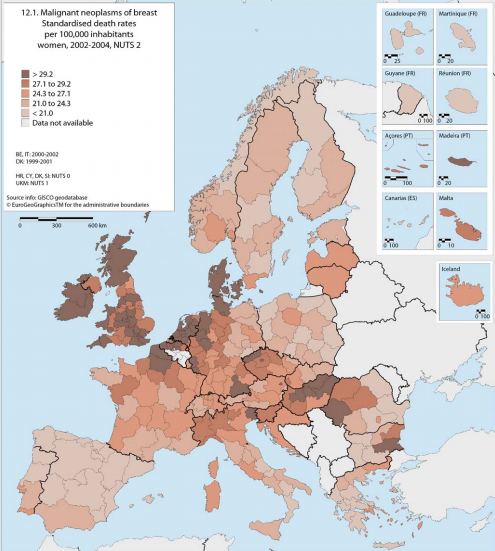
\includegraphics[scale=0.5]{Chapter1/background-img/mortality_EU_Comms.png}
  \caption{Breast tissue composition. \textit{Image Source: EU Commission: Atlas on Mortality \cite{European_Commission_2009}}}
  \label{fig:mortality-band}
\end{figure}

\subsection{Tissue density classification}

The internal breast structure consists of different kinds of tissue and glands \cite{Anatomy_breast}:

\begin{itemize}
  \item Fatty and connective tissue: protects the lobules and ducts, gives shape to the breasts
  \item Lobules - milk-production glands
  \item Ducts - carry milk from lobules to nipple
\end{itemize}

\begin{figure}[!h]
  \center
  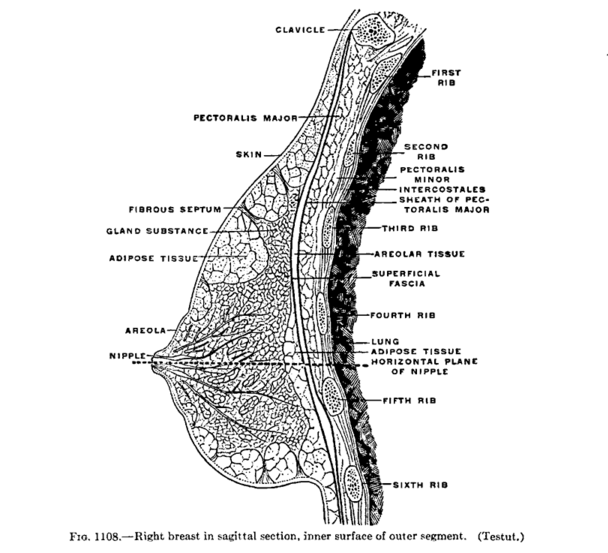
\includegraphics[scale=0.4]{Chapter1/background-img/breast_anatomy.png}
  \caption{Make up of breast structure. \textit{Image Source: Gray's Anatomy \cite{Gray_1907}}}
  \label{fig:breast-anatomy}
\end{figure}

Fatty and connective tissue density can vary widely between women. Extensive research is ongoing into the links between a higher proportion of fibrous/glandular tissue versus fatty tissue and a higher risk of breast cancer, however it is currently widely accepted there is a strong link between dense tissue and breast cancer \cite{Boyd_Byng_Jong_Fishell_Little_Miller_Lockwood_Tritchler_Yaffe_1995}. Therefore, simple classification of denser tissue is vital for both radiographers and patients alike.

There exists several methods for classifying the density of breast tissue, as outlined in the following Subsections.

\subsubsection{Wolfe classification}

Wolfe described the first qualitative means in which to classify breast tissue density in 1976 \cite{Wolfe_1976}.

\begin{itemize}
    \item \textbf{N1:} consisting mainly of fat (lowest risk)
    \item \textbf{P1:} fat plus linear densities occupying no more than 25\% of the breast (low risk)
    \item \textbf{P2:} linear densities occupying \textgreater 25\% of breast (high risk)
    \item \textbf{DY:} dense (highest risk)
\end{itemize}

\subsubsection{Boyd classification}

Boyd and colleagues proposed a quantitative means to categorising breast tissue density, based on a percentage of `dense' tissue assigned by a radiographer \cite{Boyd_Byng_Jong_Fishell_Little_Miller_Lockwood_Tritchler_Yaffe_1995}.

\begin{itemize}
  \item \textbf{A: } 0\%
  \item \textbf{B: } \textgreater 0\% - 10\%
  \item \textbf{C: } \textgreater 10\% - 25\%
  \item \textbf{D: } \textgreater 25\% - 50\%
  \item \textbf{E: } \textgreater 50\% - 75\%
  \item \textbf{F: } \textgreater 75\%
\end{itemize}

\subsubsection{BI-RADS classification}
\label{sssec:bi-rads}

A widely accepted quantitative tool for the classification and risk analysis of mammography and ultrasounds is BI-RADS (Breast Imaging-Reporting and Data System) system, defined by the American College of Radiology \cite{sickles2013acr}.

\begin{itemize}
  \item \textbf{a: } almost entirely fatty (Figure \ref{fig:birads-a})
  \item \textbf{b: } scattered areas of fibroglandular density (Figure \ref{fig:birads-b})
  \item \textbf{c: } heterogeneously dense, which may obscure small masses (Figure \ref{fig:birads-c})
  \item \textbf{d: } extremely dense, which lowers the sensitivity of mammography (Figure \ref{fig:birads-d})
\end{itemize}

\begin{figure}[!ht]
  \center
  \begin{subfigure}[ht!]{0.2\textwidth}
        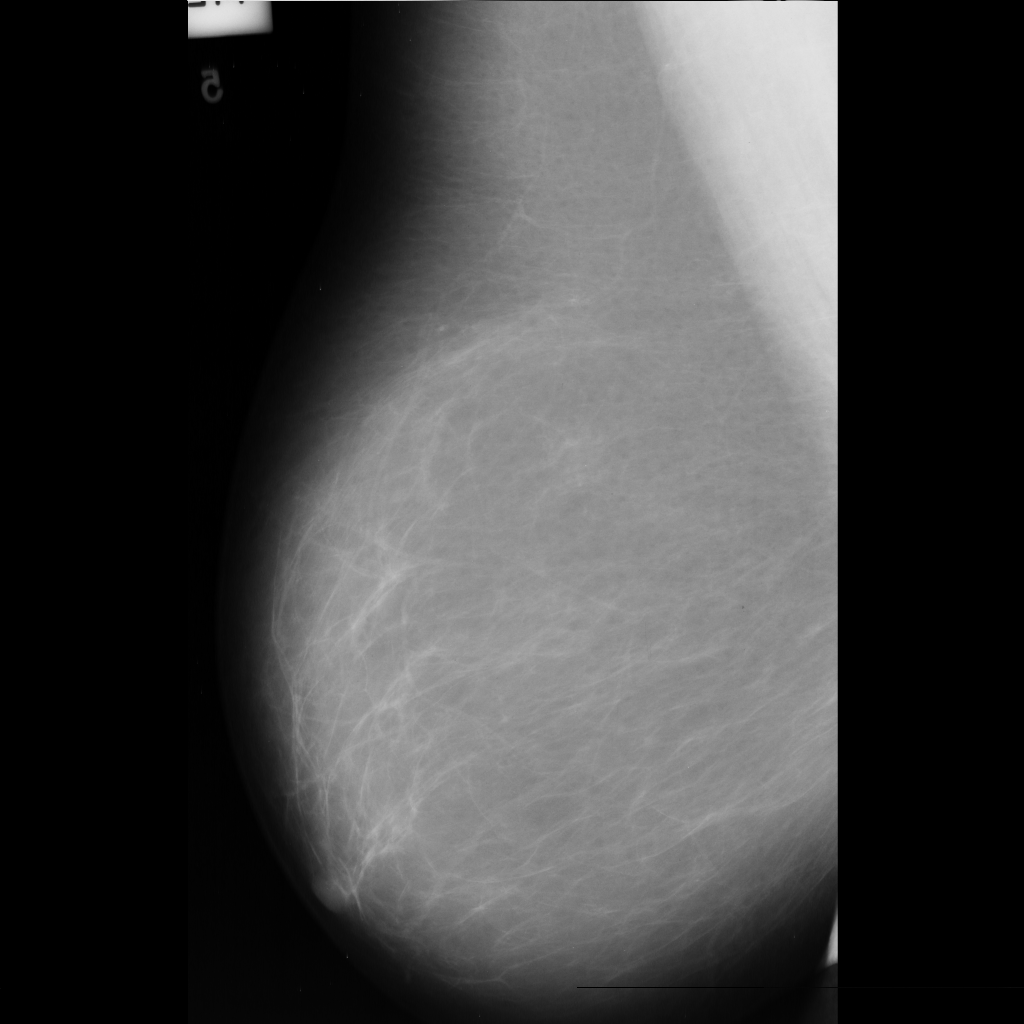
\includegraphics[width=\textwidth]{Chapter1/background-img/a.png}
        \caption{}
        \label{fig:birads-a}
    \end{subfigure}
    \begin{subfigure}[ht!]{0.2\textwidth}
          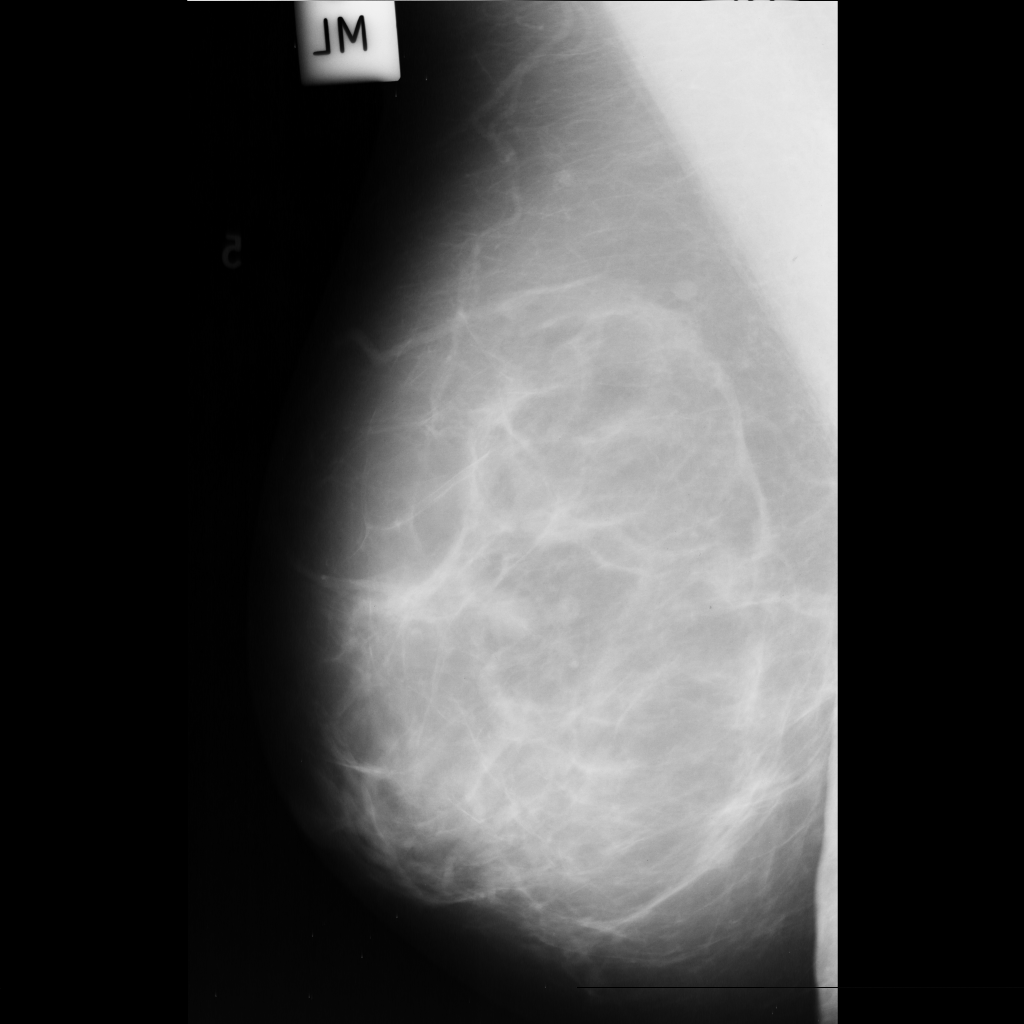
\includegraphics[width=\textwidth]{Chapter1/background-img/b.png}
          \caption{}
          \label{fig:birads-b}
    \end{subfigure}
    \begin{subfigure}[ht!]{0.2\textwidth}
          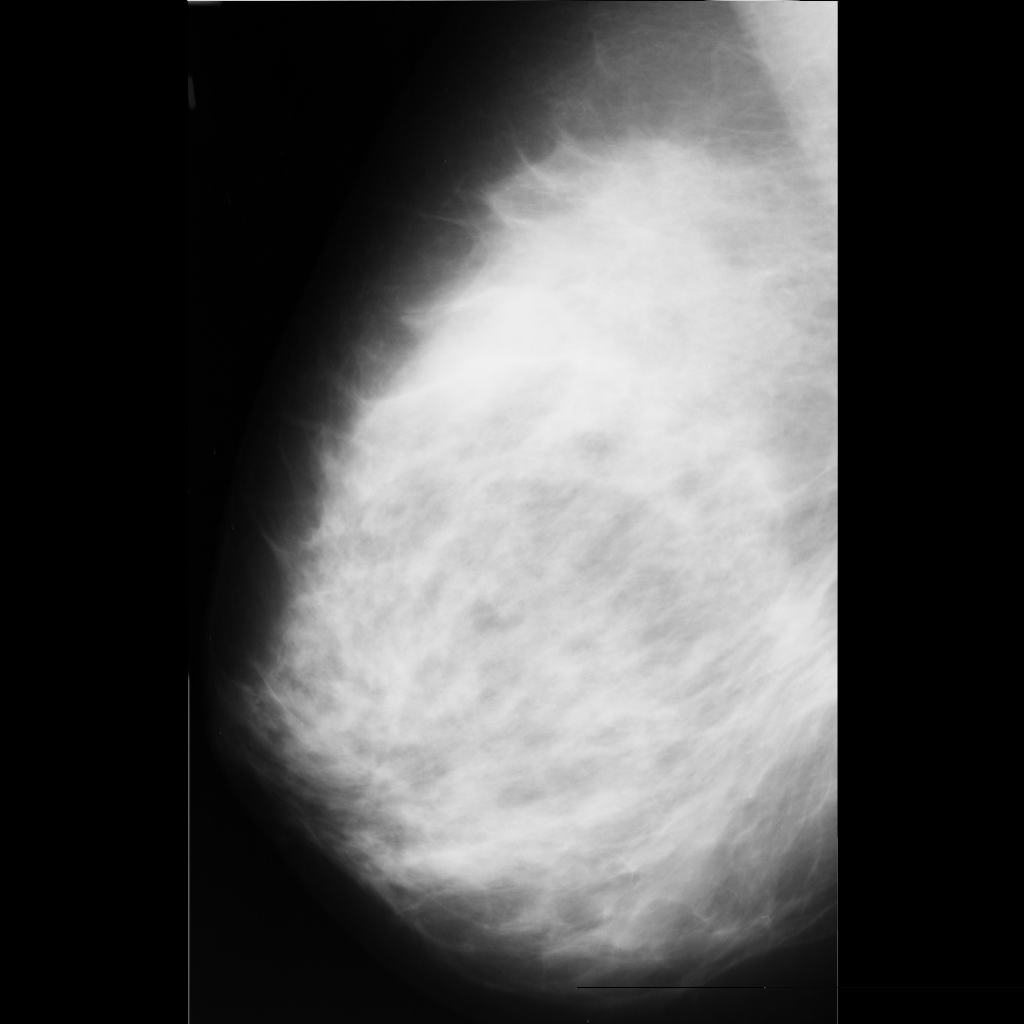
\includegraphics[width=\textwidth]{Chapter1/background-img/c.png}
          \caption{}
          \label{fig:birads-c}
    \end{subfigure}
    \begin{subfigure}[ht!]{0.2\textwidth}
          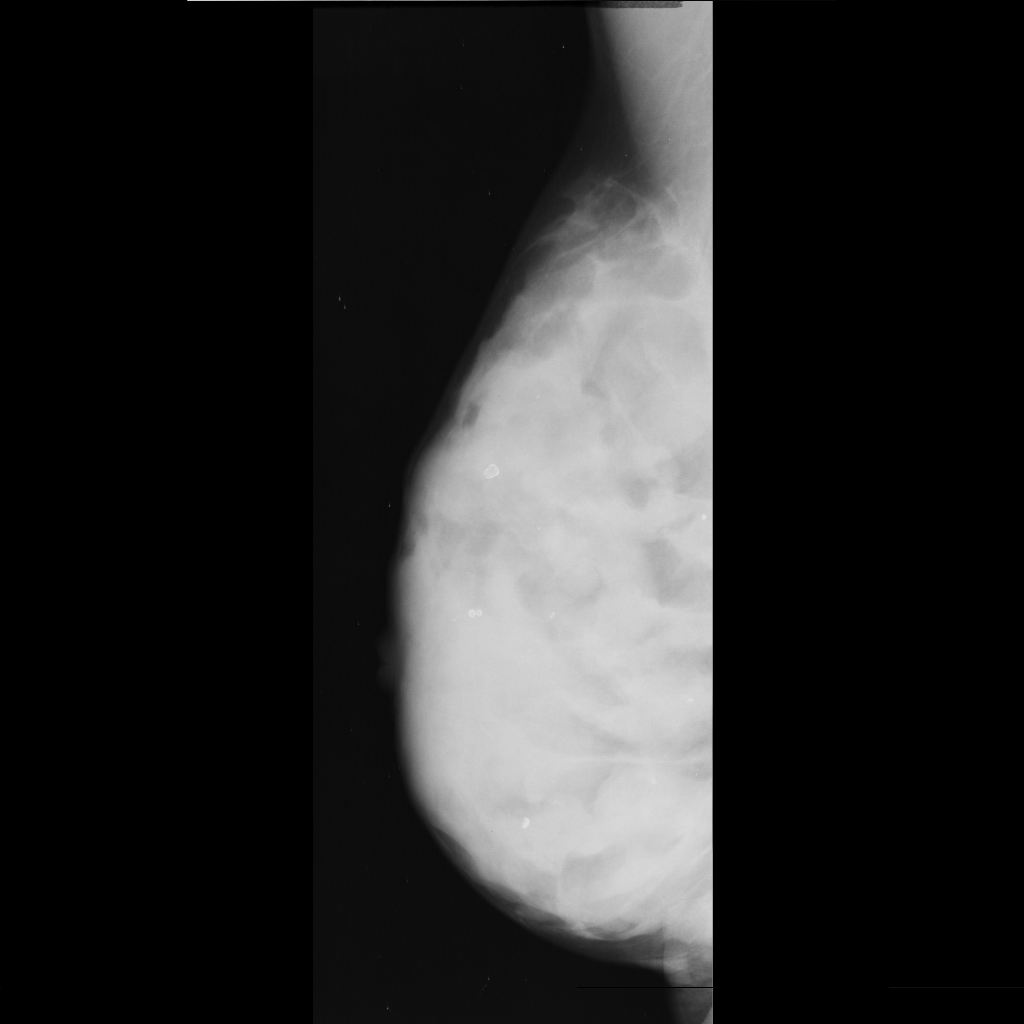
\includegraphics[width=\textwidth]{Chapter1/background-img/d.png}
          \caption{}
          \label{fig:birads-d}
    \end{subfigure}
  \caption{Comparison of the 4 BI-RADS classification}
  \label{fig:4-birads}
\end{figure}

This is the classification of choice for this project due to its wide-spread acceptance and usage in the industry.

\vspace{1cm}
\subsubsection{Tab\'ar classification}

This technique is somewhat different from the previous three by utilising anatomic-mammographic correlations, as developed by Tab\'ar \cite{al}.

\begin{itemize}
  \item \textbf{I: } balanced proportion of all components of breast tissue with a slight predominance of fibrous tissue
  \item \textbf{II: } predominance of fat tissue (fat breast)
  \item \textbf{III: } predominance of fat tissue with retroareolar residual fibrous tissue
  \item \textbf{IV: } predominantly nodular densities
  \item \textbf{V: } predominantly fibrous tissue (dense breast)
\end{itemize}

\subsection{Mammograms}

Quite simply, a Mammogram is an X-Ray of the breast tissue pressed between two plates from a number of different angles. Below are a selection of the most common angles \cite{Radswiki} \cite{Mammography_views_Doc_2016}:
\begin{itemize}
  \item Cranial-Caudal (CC) - taken from above (Figure \ref{fig:CC})
  \item Medio-Lateral Oblique (MLO) - from the side, at an angle (usually 45$\deg$) (Figure \ref{fig:MLO})
  \item Medio-Lateral (ML) - from the centre outwards (Figure \ref{fig:ML})
  \item Latero-Medial (LM) - from the side, into the centre (Figure \ref{fig:LM})
\end{itemize}

CC and MLO are generally standard practice angles, with ML and LM adding more information for the radiographer to assess.
%  \iffalse
\begin{figure}[H]
\begin{center}
  \begin{subfigure}[t]{0.45\textwidth}
    \centering
        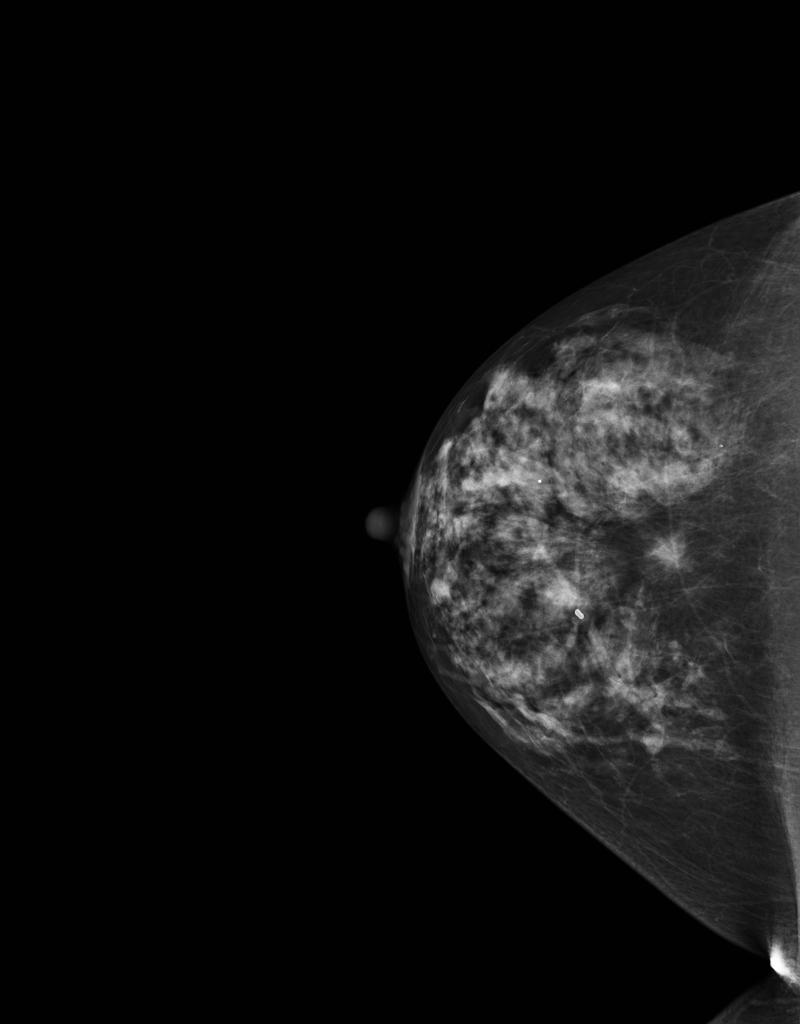
\includegraphics[height=3.5cm]{Chapter1/background-img/CC.jpg}
        \caption{Cranial-Caudal: Case courtesy of Dr Garth Kruger, Radiopaedia.org, rID: 18580}
        \label{fig:CC}
    \end{subfigure}
    \hfill
    \begin{subfigure}[t]{0.45\textwidth}
      \centering
          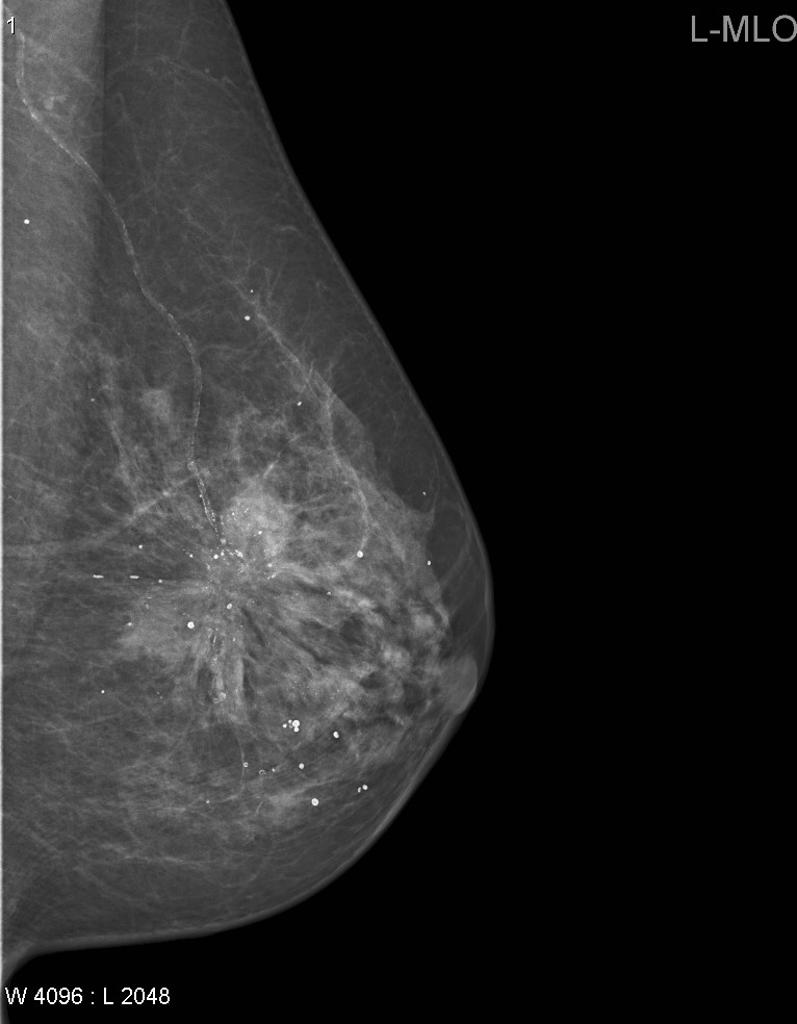
\includegraphics[height=3.5cm]{Chapter1/background-img/MLO.jpg}
          \caption{Medio-Lateral Oblique: Case courtesy of A.Prof Frank Gaillard, Radiopaedia.org, rID: 12608}
          \label{fig:MLO}
    \end{subfigure}
    \hspace*{\fill}


    \begin{subfigure}[t]{0.45\textwidth}
      \centering
          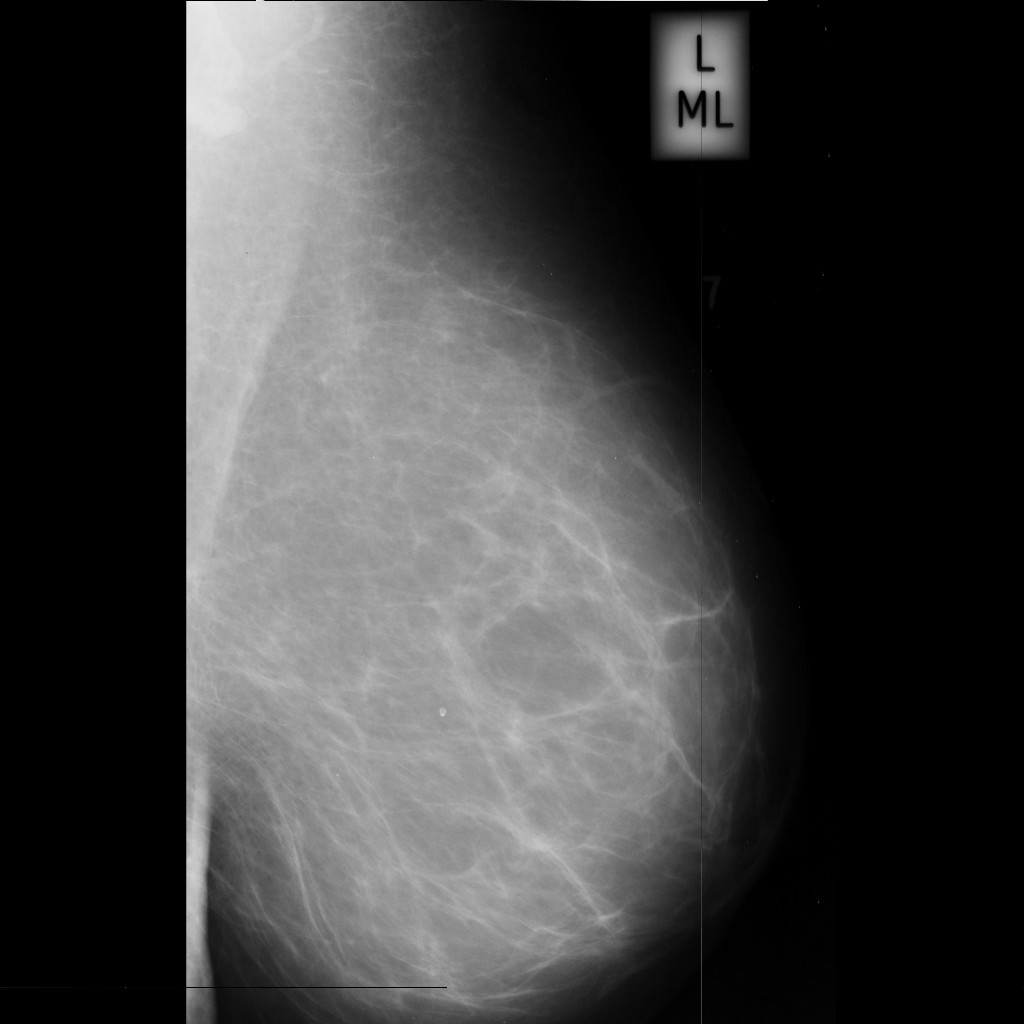
\includegraphics[height=3.5cm]{Chapter1/background-img/ML.jpg}
          \caption{Medio-Lateral: Case courtesy of Mini-MIAS dataset \cite{Suckling_1994}}
          \label{fig:LM}
    \end{subfigure}
    \hfill
    \begin{subfigure}[t]{0.45\textwidth}
      \centering
          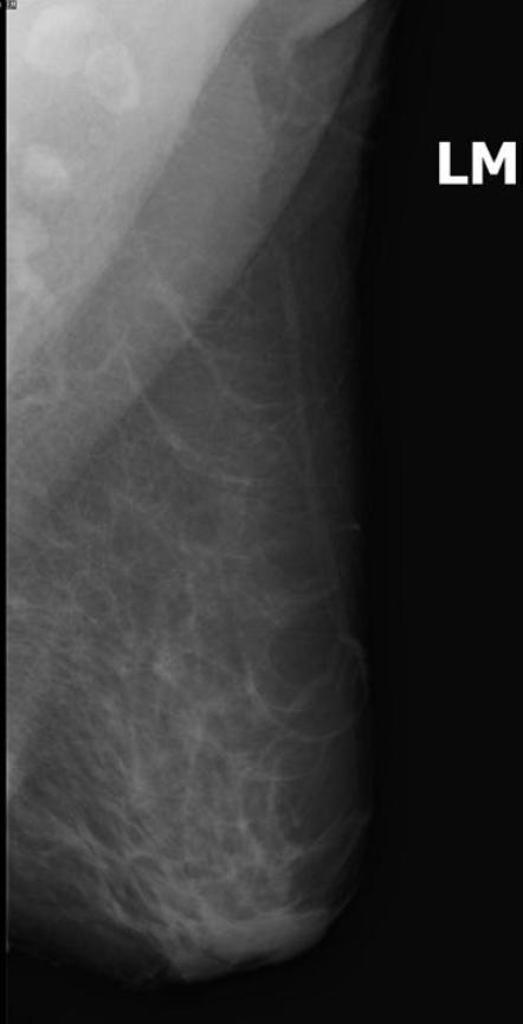
\includegraphics[height=3.5cm]{Chapter1/background-img/LM.jpg}
          \caption{Latero-Medial: Case courtesy of Dr Paresh K Desai , Radiopaedia.org, rID: 5873}
          \label{fig:ML}
    \end{subfigure}
    \hspace*{\fill}
  \caption{Comparison of the 4 mammogram angles typically used}
  \label{fig:scan-angles}
\end{center}
\end{figure}
%\fi

Organisations such as Breast Test Wales invite women between the ages of 50 and 70 to attend a scan every 3 years \cite{Informed_Choice_about_Cancer_Screening_2013}. Whilst survival rates are at an all-time high with 87\% surviving for five or more years \cite{Breast_cancer_statistics_2015}, with increased screening on high-risk patients (such as those with higher-density breasts) this percentage could be further increased.

\subsubsection{Alternatives to Mammograms}

Although the input data of choice for this project will be Mammographic images, it is important to remember that for some women, and under some circumstances, it may be more appropriate to use a different method of diagnosis.

\noindent \textbf{Ultrasound}

Women under 35 are often offered an ultrasound scan over a mammogram, due to their breasts being of a higher density naturally which makes obtaining a clear mammogram more difficult. Ultrasounds can also show the if the breast lump is a cyst, or if it is solid internally \cite{Cancer_Research_UK_2015}.

\noindent \textbf{Biopsy}

A Biopsy is usually a secondary step after diagnosis of a breast lump via mammogram or ultrasound. It can take a number of forms including:

\begin{itemize}
  \item Needle biopsy
  \item Vacuum biopsy
  \item Needle aspiration
  \item Punch biopsy
  \item Wire guided biopsy
\end{itemize}


\subsection{Existing Computer Systems}

A lot of the current computer systems focus on mammography computer aided diagnosis due to the ease in which a radiographer can misdiagnose cancer from a mammogram. Mammograms are difficult to read, or technological issues may occur, and as a result radiographers can fail to detect between 10-15\% of breast cancer cases \cite{Champaign_Cederbom_2000}.

However this is not the focus of this project. This project aims to focus upon healthy tissue, and the first steps towards computers classifying breast tissue into the correct density category. So what steps have been taken currently, in industry and in research, towards this end goal?

\todo[inline]{Paper by Mohamed Abu ElSoud; Ahmed M. Anter - Automatic mammogram segmentation and computer aided diagnoses for breast tissue density according to BIRADS dictionary}

\todo[inline]{Not sure if this section is needed? Cannot yet get ahold of above paper.}
